\begin{figure}[!htb]
	\centering
	\begin{subfigure}{0.45\textwidth}
		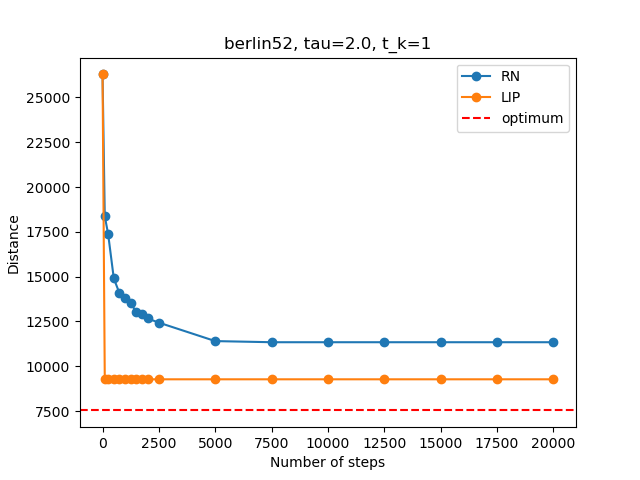
\includegraphics[width=\textwidth]{img/berlin52_temp=2.0_cool=1.0}
		\subcaption{$t_n=1$.}
	\end{subfigure}
	\begin{subfigure}{0.45\textwidth}
		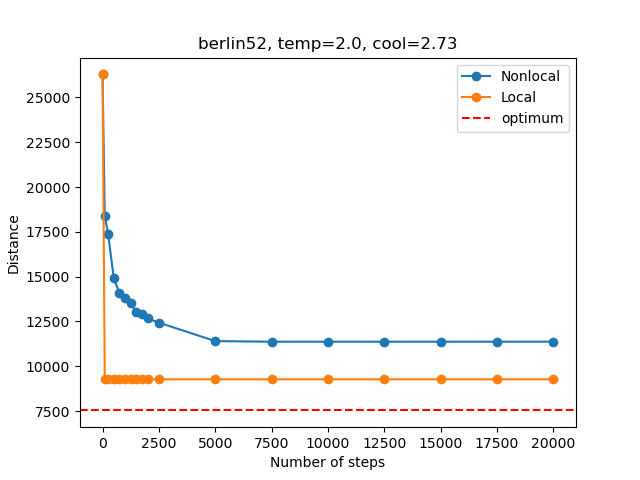
\includegraphics[width=\textwidth]{img/berlin52_temp=2.0_cool=2.73}
		\subcaption{$t_n=\frac{3}{\log(n+2)}$.}
	\end{subfigure}
	\caption{Distances over number of steps for \textit{berlin52} dataset and different cooling parameters.}
	\label{fig:berlin52_comp}
\end{figure}
	
\begin{figure}[!htb]
	\centering
	\begin{subfigure}{0.45\textwidth}
		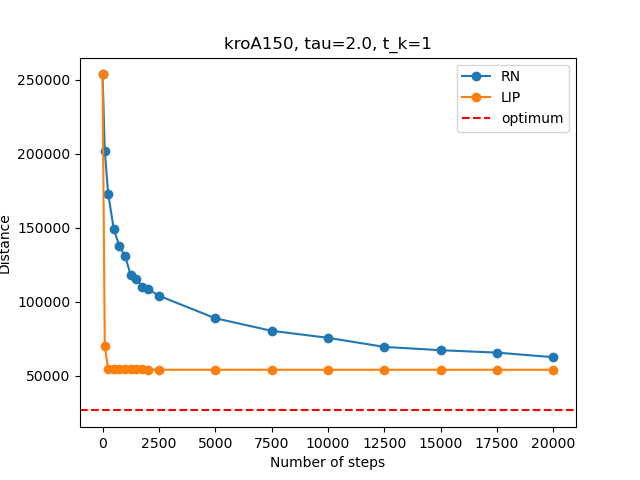
\includegraphics[width=\textwidth]{img/kroA150_temp=2.0_cool=1.0}
		\subcaption{$t_n=1$.}
	\end{subfigure}
	\begin{subfigure}{0.45\textwidth}
		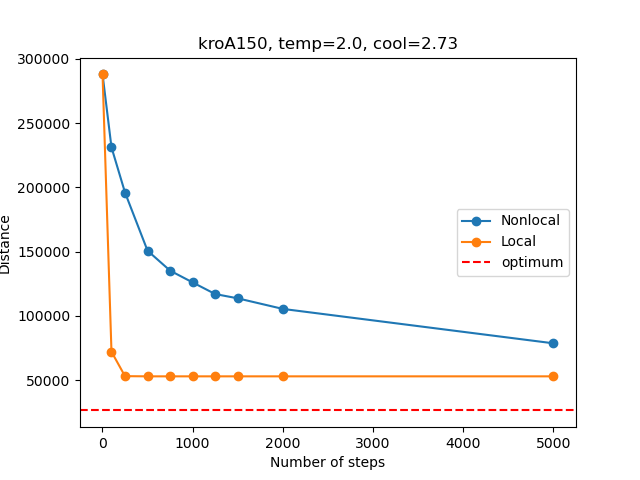
\includegraphics[width=\textwidth]{img/kroA150_temp=2.0_cool=2.73}
		\subcaption{$t_n=\frac{3}{\log(n+2)}$.}
	\end{subfigure}
	\caption{Distances over number of steps for \textit{kroA150} dataset and different cooling parameters.}
	\label{fig:kroA150_comp}
\end{figure}

\begin{figure}[!htb]
	\centering
	\begin{subfigure}{0.45\textwidth}
		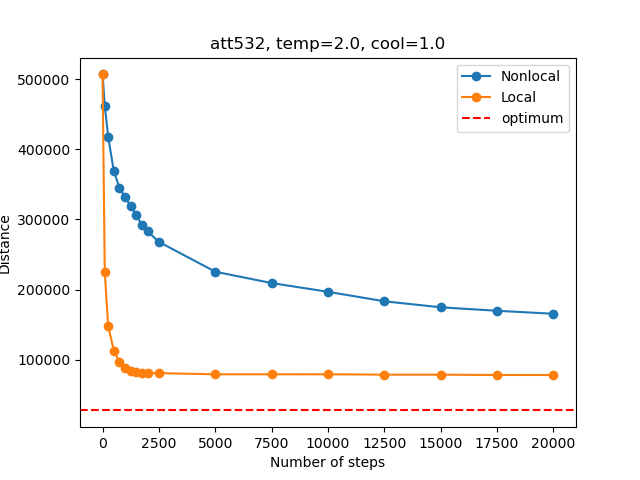
\includegraphics[width=\textwidth]{img/att532_temp=2.0_cool=1.0}
		\subcaption{$t_n=1$.}
	\end{subfigure}
	\begin{subfigure}{0.45\textwidth}
		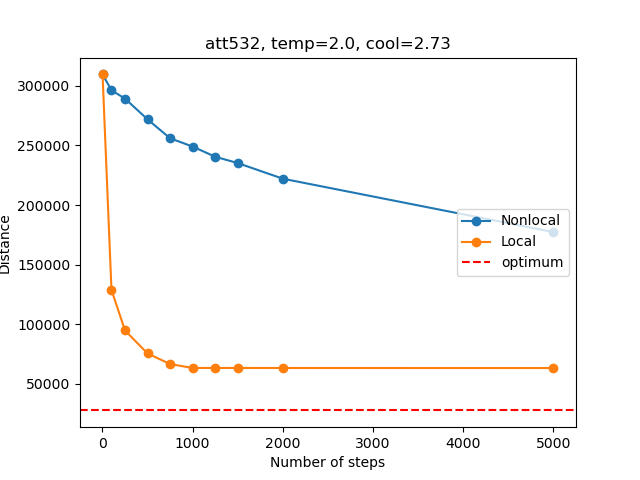
\includegraphics[width=\textwidth]{img/att532_temp=2.0_cool=2.73}
		\subcaption{$t_n=\frac{3}{\log(n+2)}$.}
	\end{subfigure}
	\caption{Distances over number of steps for \textit{att532} dataset and different cooling parameters.}
	\label{fig:att532_comp}
\end{figure}

\begin{figure}[!htb]
	\centering
	\begin{subfigure}{0.45\textwidth}
		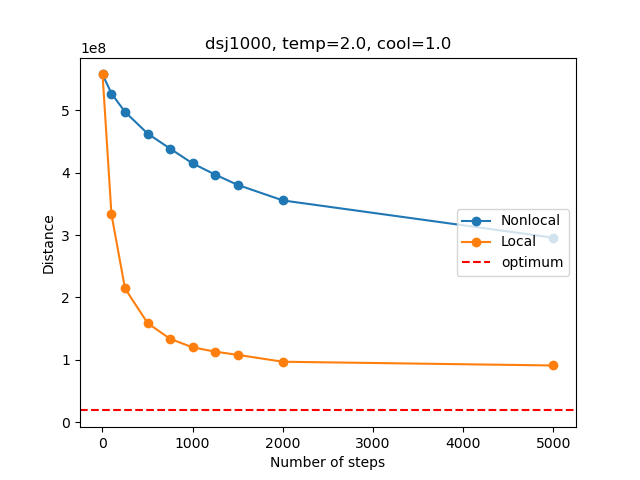
\includegraphics[width=\textwidth]{img/dsj1000_temp=2.0_cool=1.0}
		\subcaption{$t_n=1$.}
	\end{subfigure}
	\begin{subfigure}{0.45\textwidth}
		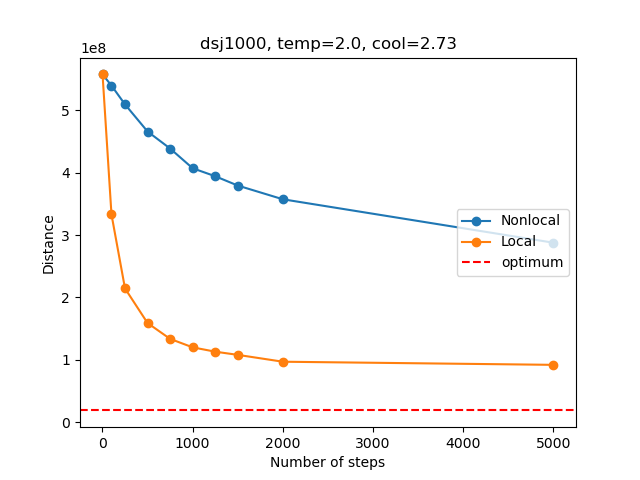
\includegraphics[width=\textwidth]{img/dsj1000_temp=2.0_cool=2.73}
		\subcaption{$t_n=\frac{3}{\log(n+2)}$.}
	\end{subfigure}
	\caption{Distances over number of steps for \textit{dsj1000} dataset and different cooling parameters.}
	\label{fig:dsj1000_comp}
\end{figure}